\chapter{Marco Teórico}
\label{ch:marco_teorico}

\section{Introducción}
\label{sec:intro_marco_teorico}

Una vez delimitados en el Capítulo \ref{cap:objetivos_alcance_antecedentes} los objetivos de la investigación y las limitaciones documentadas en la literatura frente a las que se posiciona este trabajo, el presente capítulo desarrolla de manera formal el fundamento matemático y algorítmico sobre el que se sustenta la propuesta. La exposición se organiza en tres bloques progresivos: en primer lugar, se establece la transformación matemática que traslada el problema financiero de selección de carteras desde su formulación continua de Markowitz hasta un Hamiltoniano de Ising instanciable en un registro de cúbits; en segundo lugar, se analiza críticamente la arquitectura de circuito del QAOA estándar, se identifican sus limitaciones estructurales y se presenta la arquitectura alternativa con preservación de simetría propuesta en este trabajo; y en tercer lugar, se describen los mecanismos de estabilización de la optimización clásica que complementan dicha arquitectura.

A diferencia del Capítulo \ref{cap:desarrollo_metodologia}, que detalla la instanciación concreta de estos elementos sobre datos reales —incluyendo el origen de los datos financieros, las herramientas de software empleadas y la justificación numérica de cada hiperparámetro—, el presente capítulo se limita a establecer su fundamento matemático y su justificación teórica, independiente de cualquier instancia particular del problema.

\section{Formulación Matemática}
\label{sec:formulacion_matematica}

\subsection{El Modelo Continuo de Media-Varianza}
\label{subsec:modelo_media_varianza}

El punto de partida analítico de este trabajo es el modelo de media-varianza de Markowitz \cite{Markowitz1952}, que evalúa el compromiso entre el retorno esperado de una cartera de inversión y su riesgo asociado. Dado un universo de $N$ activos financieros, con un vector de pesos de capital $w \in \mathbb{R}^N$ asignado a cada uno de ellos, el retorno esperado de la cartera se define como:
\begin{equation}
    \mu_p = \sum_{i=1}^{N} w_i \mu_i
    \label{eq:retorno_cartera}
\end{equation}
donde $\mu_i$ denota el retorno esperado individual del activo $i$. De forma análoga, el riesgo de la cartera se cuantifica a través de su varianza:
\begin{equation}
    \sigma_p^2 = \sum_{i=1}^{N} \sum_{j=1}^{N} w_i w_j \sigma_{ij}
    \label{eq:riesgo_cartera}
\end{equation}
siendo $\sigma_{ij}$ el elemento $(i,j)$ de la matriz de covarianza $\Sigma \in \mathbb{R}^{N \times N}$ de los retornos de los activos. El problema de optimización clásico busca, por tanto, un equilibrio entre maximizar $\mu_p$ y minimizar $\sigma_p^2$, dando lugar a la conocida frontera eficiente de carteras óptimas.

\subsection{Formulación QUBO}
\label{subsec:discretizacion_qubo}

Para adaptar el modelo continuo a una arquitectura cuántica basada en cúbits, es necesario introducir variables de decisión binarias $x_i \in \{0,1\}$, donde $x_i = 1$ indica la inclusión del activo $i$ en la cartera y $x_i = 0$ su exclusión. Bajo una estrategia de equiponderación con cardinalidad fija $K$, el peso de cada activo seleccionado se define como:
\begin{equation}
    w_i = \frac{x_i}{K}
    \label{eq:peso_equiponderado}
\end{equation}
Esta elección de equiponderación, en lugar de permitir pesos continuos arbitrarios sobre los activos seleccionados, mantiene el problema estrictamente en el dominio combinatorio: la única decisión que debe resolver el algoritmo es \emph{qué} $K$ activos incluir, no en qué proporción exacta ponderarlos, lo cual es coherente con el objetivo de este trabajo de evaluar la capacidad de los algoritmos cuánticos variacionales para resolver problemas de selección combinatoria pura.

La restricción de cardinalidad exacta $\sum_{i=1}^N x_i = K$ constituye una restricción dura del problema. Sin embargo, la formulación de Optimización Binaria Cuadrática No Restringida (QUBO, por sus siglas en inglés) exige, por definición, la ausencia de restricciones explícitas. Por ello, dicha restricción debe incorporarse directamente en la función objetivo mediante un término de penalización cuadrática:
\begin{equation}
    P \left( \sum_{i=1}^N x_i - K \right)^2
    \label{eq:penalizacion_cardinalidad}
\end{equation}
donde $P$ es un multiplicador escalar de penalización. Este término alcanza su valor mínimo (cero) exclusivamente cuando la restricción de cardinalidad se satisface de forma exacta, y crece cuadráticamente ante cualquier desviación.

Integrando las Ecuaciones \eqref{eq:peso_equiponderado} y \eqref{eq:penalizacion_cardinalidad} en el objetivo de media-varianza, se obtiene la función de coste QUBO completa del problema:
\begin{equation}
    Q(x) = \lambda \, w^T \Sigma w - (1-\lambda)\, \mu^T w
    + P \left( \sum_{i=1}^N x_i - K \right)^2
    \label{eq:qubo_completo}
\end{equation}
donde $\lambda \in [0,1]$ es el parámetro de aversión al riesgo que pondera la importancia relativa de la minimización de varianza frente a la maximización de retorno. Para que la penalización cumpla su función, el multiplicador $P$ debe dominar en magnitud al resto de términos del objetivo, de modo que cualquier configuración binaria factible (con exactamente $K$ activos seleccionados) tenga siempre una energía menor que cualquier configuración infactible, independientemente de la calidad financiera de esta última. El criterio numérico concreto empleado para fijar $P$ en las instancias experimentales de este trabajo se detalla en el Capítulo \ref{cap:desarrollo_metodologia}.

La expansión algebraica completa de la Ecuación \eqref{eq:qubo_completo} da lugar a una matriz $Q \in \mathbb{R}^{N \times N}$ simétrica, cuyos elementos diagonales y fuera de la diagonal codifican, respectivamente, las contribuciones individuales de cada activo y las interacciones cuadráticas entre pares de activos. Esta matriz $Q$ constituye la representación QUBO íntegra del problema financiero discretizado.

\subsection{Mapeo al Hamiltoniano de Ising}
\label{subsec:mapeo_ising}

Para trasladar el problema QUBO al dominio de la mecánica cuántica, es necesario expresarlo en términos de operadores de espín de Pauli. Esto se logra mediante la transformación afín que relaciona cada variable binaria $x_i$ con el operador $Z_i$ de Pauli, cuyos autovalores son $\{-1, +1\}$:
\begin{equation}
    x_i = \frac{I - Z_i}{2}
    \label{eq:transformacion_spin}
\end{equation}
Sustituyendo la Ecuación \eqref{eq:transformacion_spin} en la función de coste QUBO de la Ecuación \eqref{eq:qubo_completo} y reagrupando términos, la función objetivo se reescribe como un Hamiltoniano de Ising:
\begin{equation}
    H_P = \sum_{i=1}^N h_i Z_i + \sum_{i=1}^N \sum_{j > i}^N J_{ij} Z_i Z_j + O_{\text{ffset}}
    \label{eq:hamiltoniano_ising}
\end{equation}
En esta expresión, los coeficientes $J_{ij}$ —que representan los acoplamientos ponderados entre pares de cúbits— quedan determinados por los elementos fuera de la diagonal de la matriz de covarianza $\Sigma$, mientras que los campos locales $h_i$ quedan determinados por una combinación del vector de retornos esperados $\mu$ y de la contribución lineal que surge al expandir el término de penalización de cardinalidad de la Ecuación \eqref{eq:penalizacion_cardinalidad}. El término $O_{\text{ffset}}$ es una constante aditiva sin relevancia física para la determinación del estado fundamental, puesto que no afecta a la posición del mínimo de energía.

De este modo, el problema de selección de carteras bajo restricción de cardinalidad exacta queda formalmente traducido a la búsqueda del estado fundamental de un sistema de espines acoplados, es decir, a la determinación de la configuración de espines $\{Z_i\}$ que minimiza la energía $H_P$.

Este flujo de traducción estructural, desde los datos financieros de entrada hasta la instanciación de la red de espines, se esquematiza en la Figura \ref{fig:diagrama_mapeo}.

\begin{figure}[htbp]
    \centering
    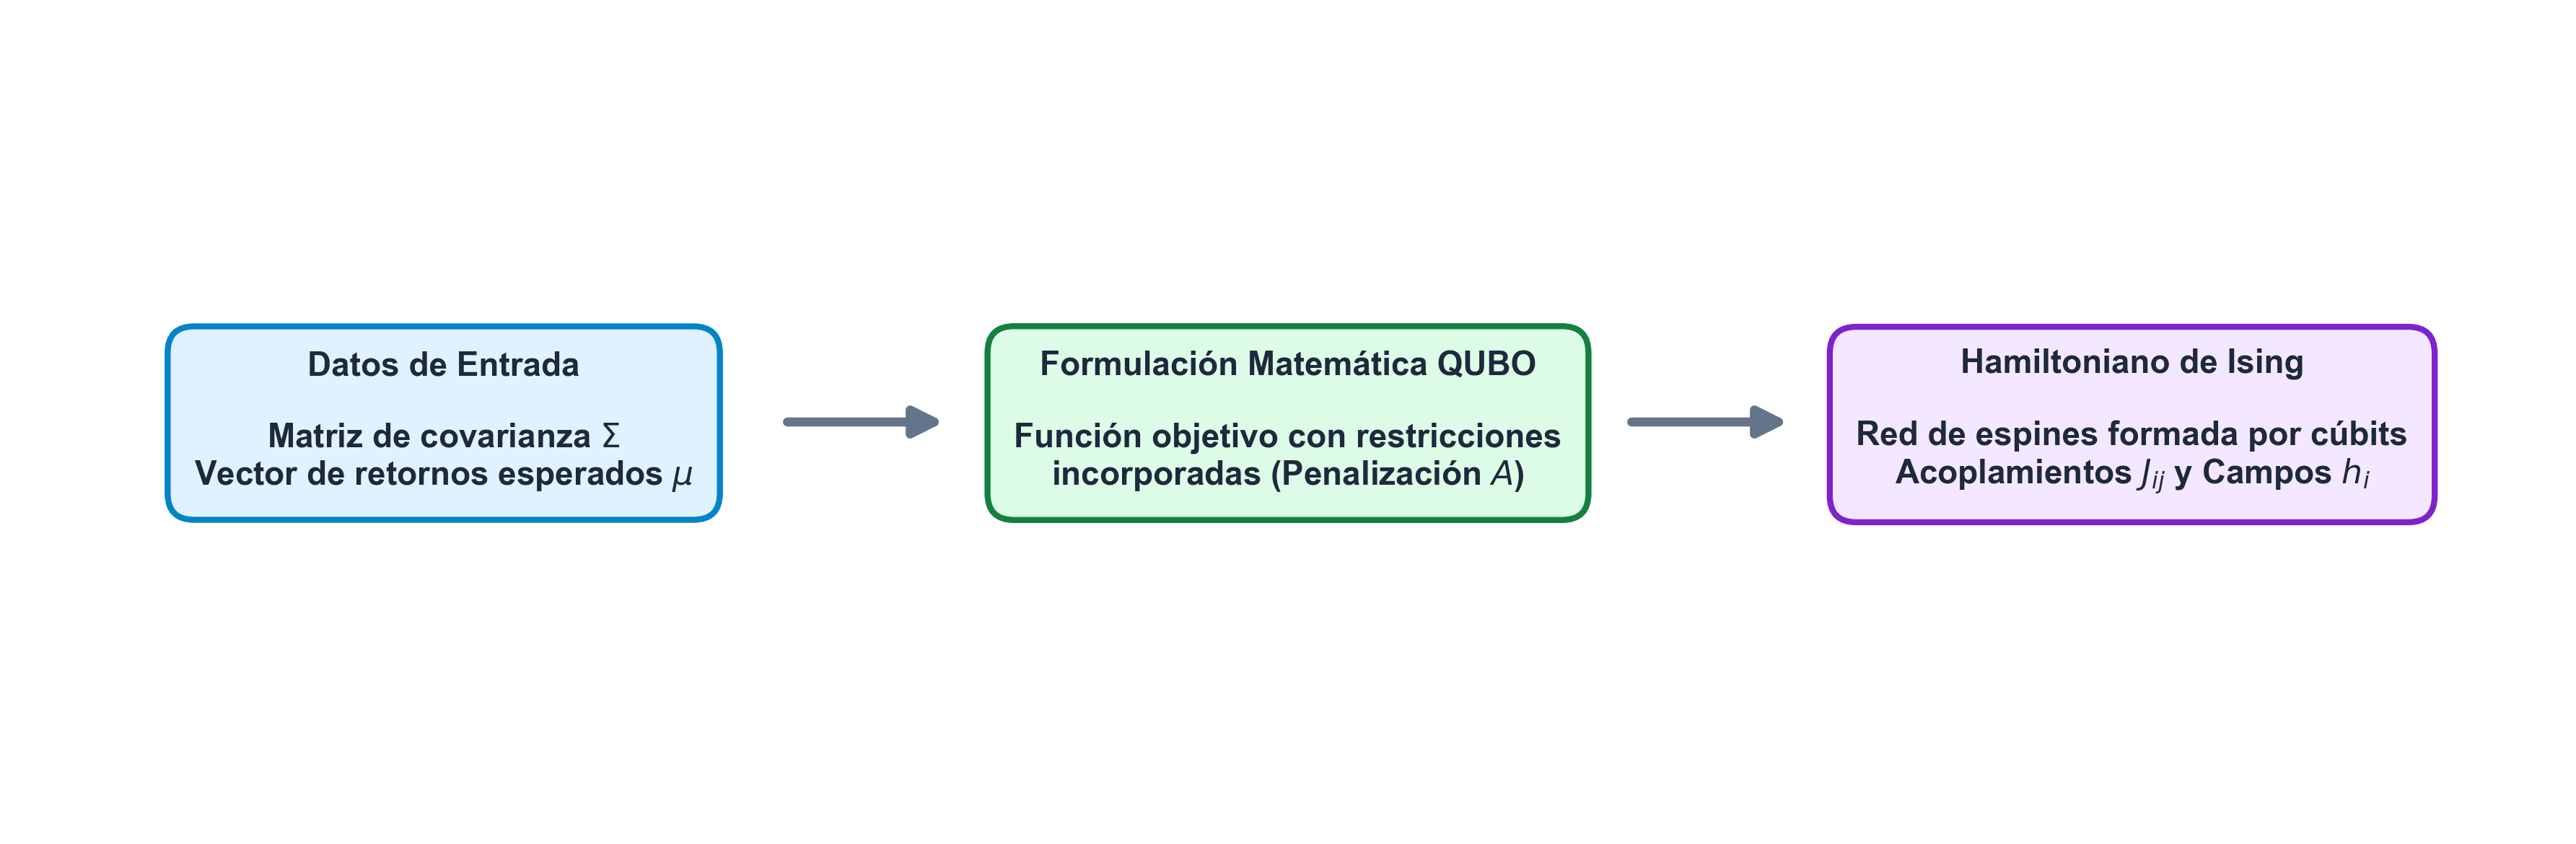
\includegraphics[width=0.95\textwidth]{output/figures/diagrama_flujo_mapeo.png}
    \caption{Diagrama de flujo conceptual del mapeo matemático}
    \label{fig:diagrama_mapeo}
\end{figure}

\section{Arquitectura Cuántica}
\label{sec:arquitectura_cuantica}

\subsection{QAOA Estándar y el Mezclador Transversal}
\label{subsec:qaoa_estandar}

Retomando la estructura general de QAOA introducida en el Capítulo
\ref{ch:introduccion}, cada una de las $p$ capas del circuito aplica
sucesivamente el operador de coste $U_C(\gamma) = e^{-i\gamma H_P}$,
que codifica el Hamiltoniano de Ising definido en la Ecuación
\eqref{eq:hamiltoniano_ising}, y un operador mezclador
$U_M(\beta) = e^{-i\beta H_M}$, encargado de redistribuir la amplitud de
probabilidad entre los estados de la base computacional.

En su formulación estándar, el Hamiltoniano mezclador se define como la suma de los operadores de rotación de bit ($X$) sobre cada cúbit del registro:
\begin{equation}
    H_M = \sum_{i=1}^N X_i
    \label{eq:mezclador_x}
\end{equation}
Este operador conecta entre sí, mediante transiciones directas, la totalidad de los estados de la base computacional. En consecuencia, la evolución generada por $U_M(\beta)$ bajo el mezclador transversal explora de forma indiscriminada el espacio de Hilbert completo, de dimensión $2^N$, incluyendo un elevado número de configuraciones que violan la restricción de cardinalidad $\sum_i x_i = K$. Bajo esta arquitectura, la única vía disponible para disuadir al circuito de converger hacia dichas configuraciones infactibles es incrementar la magnitud del multiplicador de penalización $P$ definido en la Ecuación \eqref{eq:penalizacion_cardinalidad}, lo cual, como se desarrolla a continuación, introduce una patología adicional en el proceso de optimización clásica.

\subsection{Deformación del Paisaje y Barren Plateaus}
\label{subsec:barren_plateaus}

El incremento del multiplicador $P$ necesario para garantizar la factibilidad de las soluciones bajo el mezclador estándar tiene un efecto directo sobre la geometría del paisaje energético $\langle H_P \rangle (\gamma, \beta)$ que debe recorrer el optimizador clásico. Al introducir un término cuya magnitud domina ampliamente al resto de contribuciones del objetivo financiero, el paisaje de coste desarrolla gradientes de magnitud extremadamente dispar entre las regiones asociadas a configuraciones factibles e infactibles, lo cual dificulta severamente la tarea del optimizador local.

Este fenómeno se relaciona directamente con el problema, documentado en la literatura de aprendizaje cuántico variacional, de las denominadas mesetas estériles o \textit{Barren Plateaus} \cite{McClean2018}. McClean \textit{et al.} demostraron que, para circuitos variacionales suficientemente expresivos, la varianza del gradiente de la función de coste respecto a los parámetros del circuito decae exponencialmente con el número de cúbits del registro:
\begin{equation}
    \text{Var}\left[ \partial_\theta \langle H \rangle \right] \sim \mathcal{O}\left(\frac{1}{2^N}\right)
    \label{eq:barren_plateau_scaling}
\end{equation}
Esta caída exponencial de la varianza del gradiente produce regiones extensas del paisaje de optimización en las que el gradiente es, a efectos numéricos, indistinguible de cero, impidiendo que optimizadores locales sin gradiente como COBYLA o SLSQP progresen de forma efectiva hacia el óptimo. La combinación de penalizaciones de gran magnitud y el fenómeno de mesetas estériles constituye, por tanto, una doble patología estructural del QAOA estándar aplicado a problemas con restricciones duras. Este comportamiento se ilustra conceptualmente en la Figura \ref{fig:barren_plateaus}.

\begin{figure}[htbp]
    \centering
    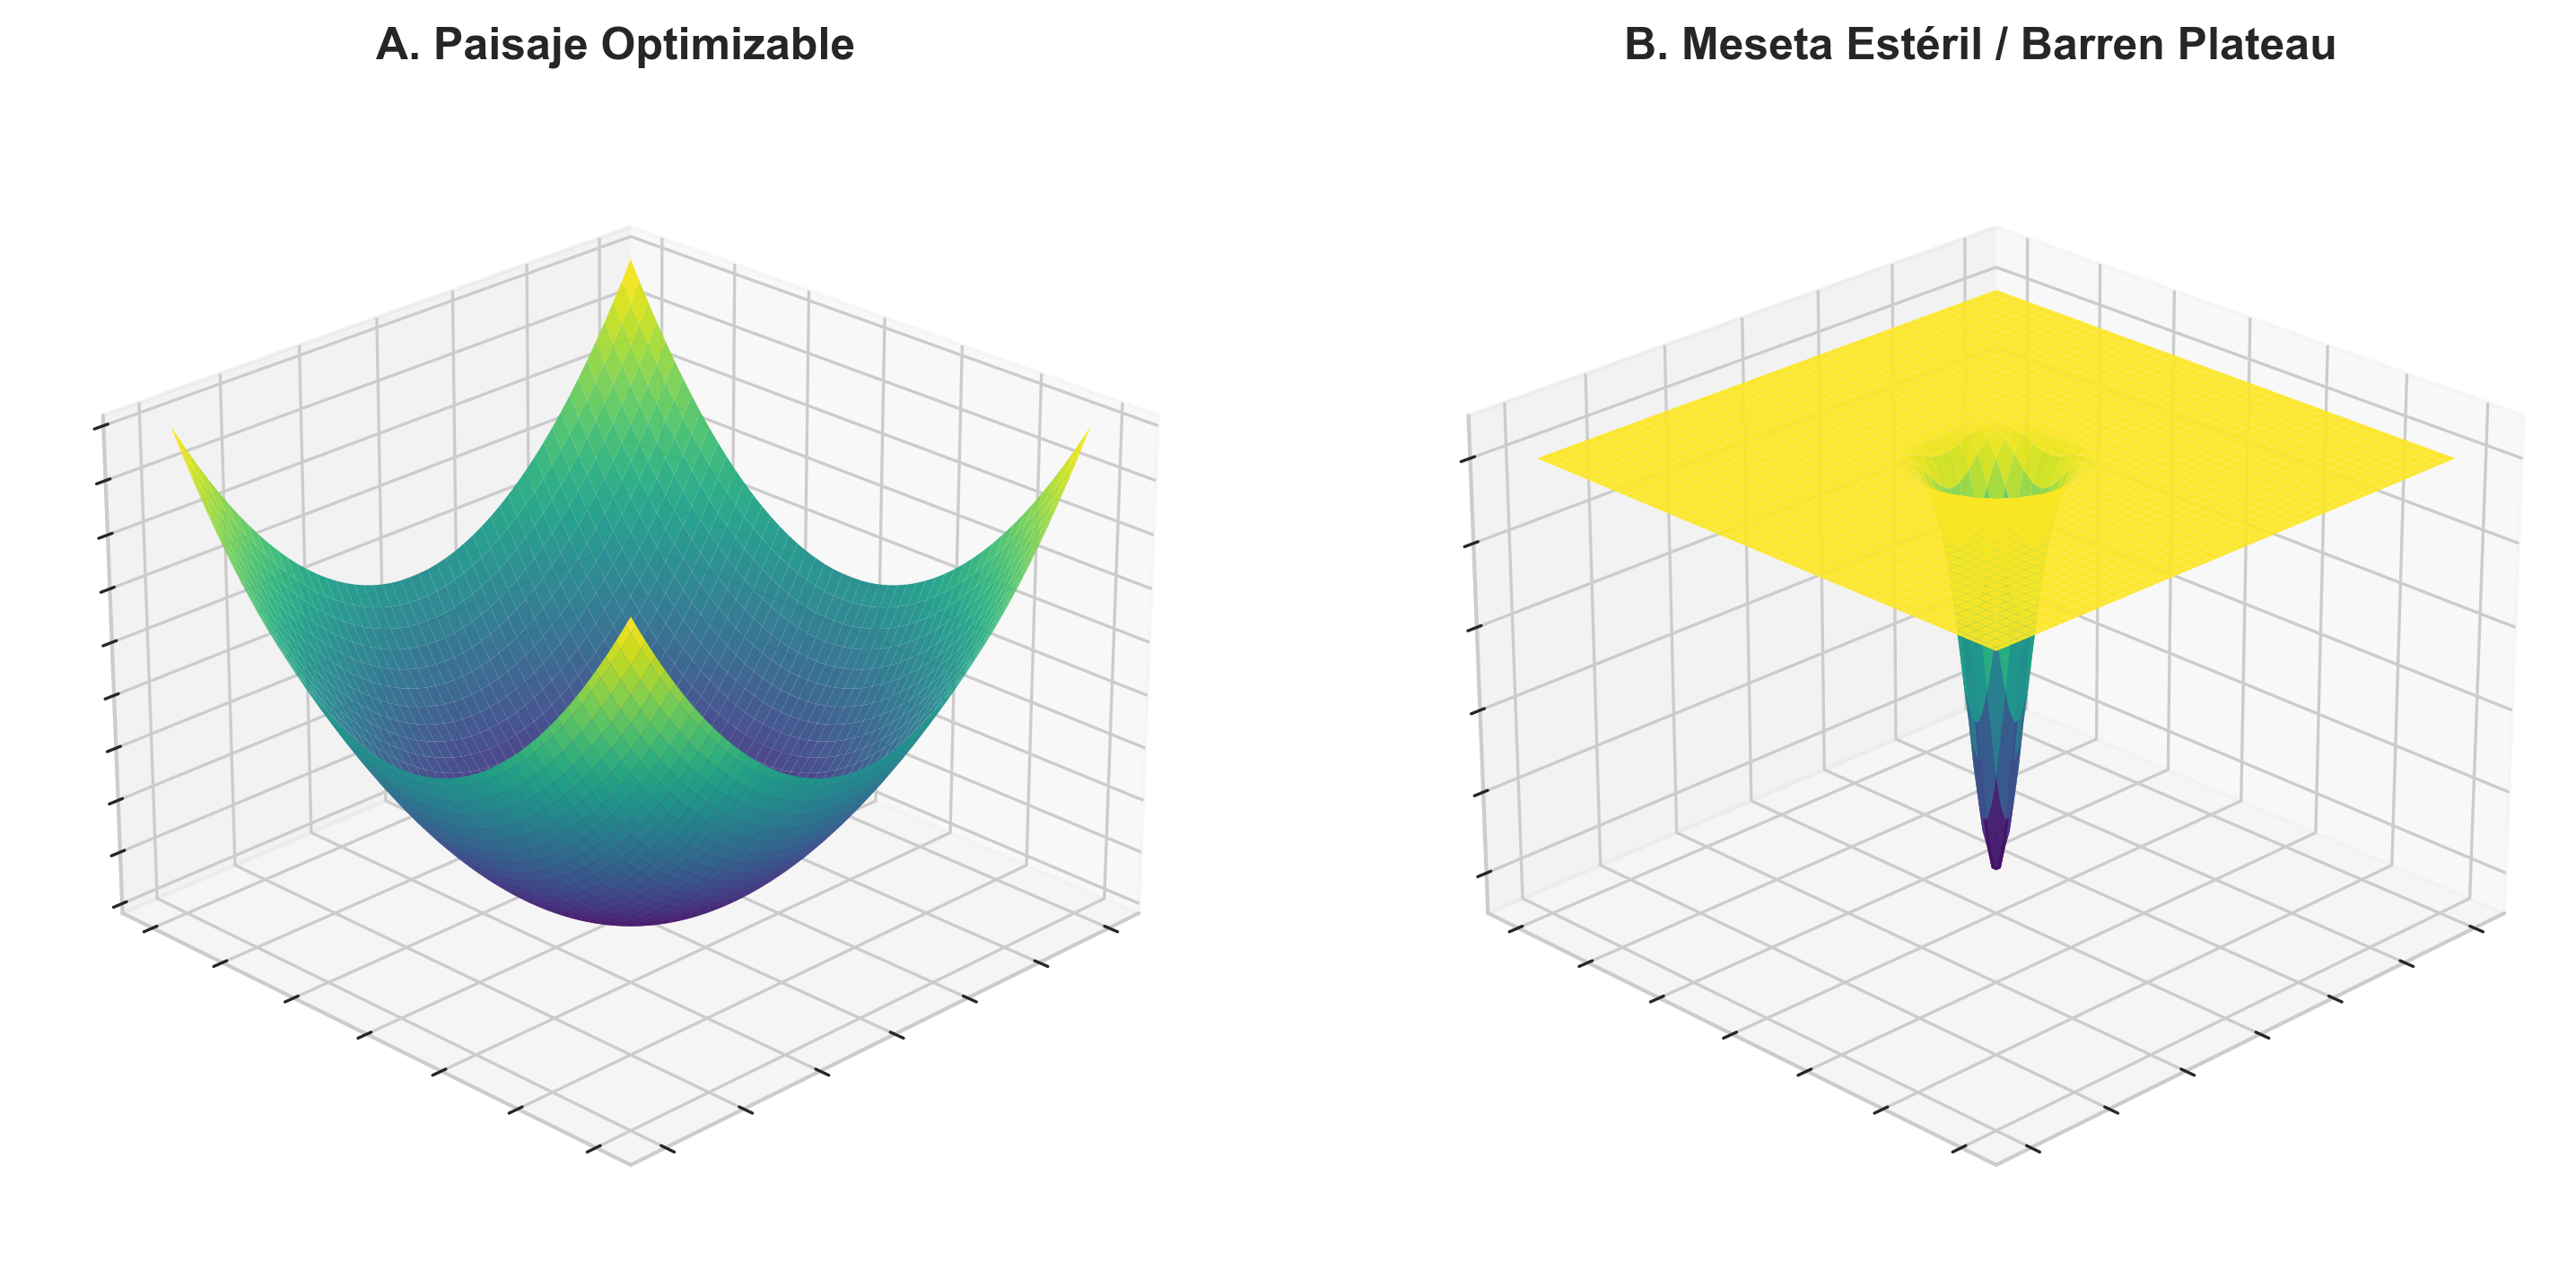
\includegraphics[width=0.95\textwidth]{output/figures/barren_plateaus.png}
    \caption{Representación conceptual del impacto de la varianza del gradiente en algoritmos variacionales.}
    \label{fig:barren_plateaus}
\end{figure}

Ante esta doble patología —exploración de estados infactibles y desvanecimiento del gradiente—, se plantea sustituir el mezclador transversal por un operador que confine la dinámica cuántica de forma nativa al subespacio factible, sin necesidad de penalización alguna. Las dos secciones siguientes desarrollan esta alternativa.

\subsection{Estados de Dicke y Confinamiento Combinatorio}
\label{subsec:estados_dicke}

Un estado de Dicke $|D_K^N\rangle$ se define como la superposición cuántica uniforme de todas las configuraciones de la base computacional de $N$ cúbits que poseen exactamente $K$ cúbits en el estado $|1\rangle$:
\begin{equation}
    |D_K^N\rangle = \binom{N}{K}^{-1/2} \sum_{\substack{x \in \{0,1\}^N \\ |x|=K}} |x\rangle
    \label{eq:estado_dicke}
\end{equation}
donde $|x|$ denota el peso de Hamming de la cadena de bits $x$, es decir, el número de unos que contiene. Si el circuito cuántico se inicializa directamente en $|D_K^N\rangle$, en lugar de en la superposición uniforme $|+\rangle^{\otimes N}$ empleada por el QAOA estándar, y el operador mezclador utilizado preserva el peso de Hamming del estado a lo largo de toda la evolución (propiedad que se demuestra en la Sección \ref{subsec:mezclador_xy}), la dinámica completa del circuito queda confinada al subespacio de dimensión $\binom{N}{K}$, en lugar del espacio de Hilbert completo de dimensión $2^N$.

El impacto cuantitativo de este confinamiento combinatorio sobre distintos tamaños de universo de activos $N$ y cardinalidades $K$ se recoge en la Tabla \ref{tab:dimension_espacio} del Capítulo \ref{ch:introduccion}. La reducción del espacio de búsqueda ilustrada en dicha tabla se representa de forma esquemática en la Figura \ref{fig:espacio_dicke}.

\begin{figure}[htbp]
    \centering
    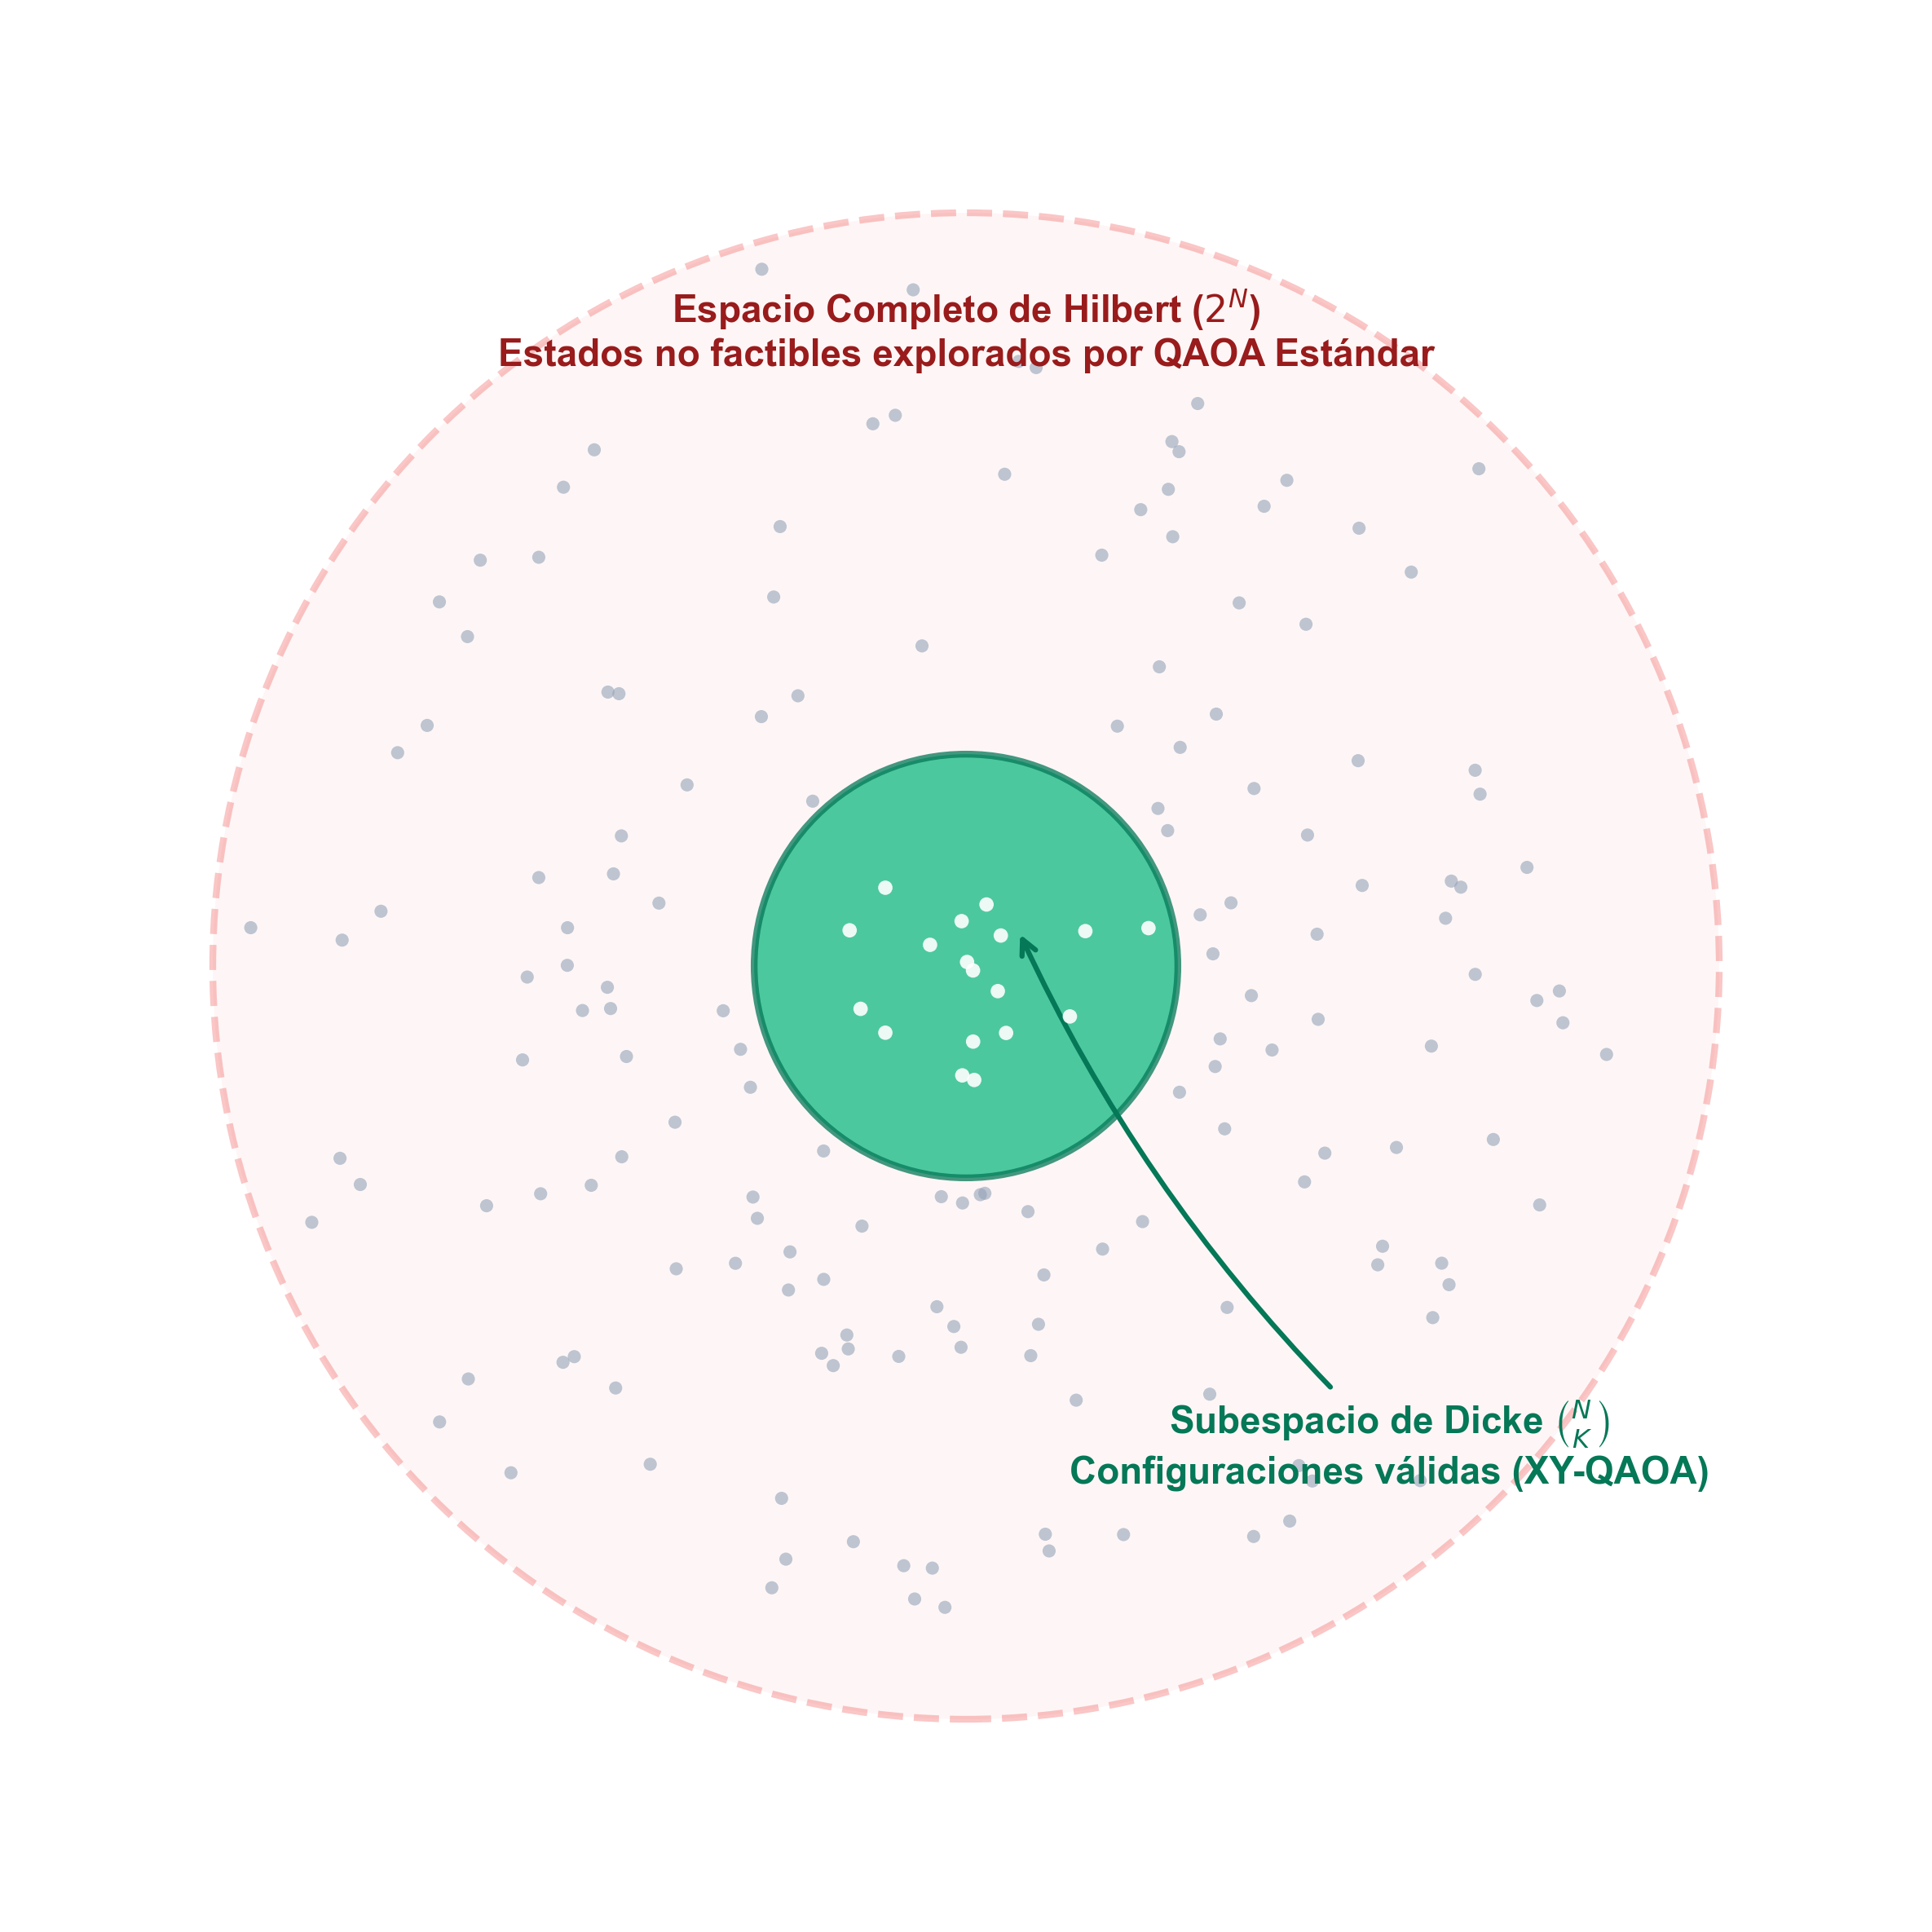
\includegraphics[width=0.85\textwidth]{output/figures/espacio_dicke_combinatorio.png}
    \caption{Representación conceptual de la reducción de la dimensionalidad combinatoria.}
    \label{fig:espacio_dicke}
\end{figure}

\subsection{El Operador de Mezcla XY y su Conmutación con el Peso de Hamming}
\label{subsec:mezclador_xy}

Para que la inicialización en el estado de Dicke resulte efectiva, es necesario sustituir el mezclador transversal de la Ecuación \eqref{eq:mezclador_x} por un operador cuya evolución preserve el peso de Hamming del estado cuántico durante toda la ejecución del circuito. Este trabajo emplea, con este propósito, el operador de mezcla basado en interacciones de intercambio de espín XY:
\begin{equation}
    H_{M}^{XY} = \frac{1}{2} \sum_{\langle i,j \rangle} \left( X_i X_j + Y_i Y_j \right)
    \label{eq:mezclador_xy}
\end{equation}
donde la suma se extiende sobre los pares de cúbits $\langle i,j \rangle$ acoplados según la topología física del circuito. Físicamente, este operador permuta las amplitudes de probabilidad entre dos cúbits únicamente cuando estos se encuentran en estados opuestos, es decir, actúa de forma no trivial sobre el subespacio generado por $\{|01\rangle, |10\rangle\}$, dejando invariantes los estados $|00\rangle$ y $|11\rangle$.

Esta propiedad físico se traduce en el resultado matemático central que justifica la arquitectura propuesta en este trabajo: el operador $H_M^{XY}$ conmuta con el operador de peso de Hamming del sistema, expresado en términos de espín como $\sum_i Z_i$:
\begin{equation}
    \left[ H_{M}^{XY}, \sum_{i=1}^N Z_i \right] = 0
    \label{eq:conmutador_xy}
\end{equation}
La conmutación establecida en la Ecuación \eqref{eq:conmutador_xy} implica que $H_M^{XY}$ y $\sum_i Z_i$ admiten una base común de autoestados. En consecuencia, cualquier evolución unitaria generada por $H_M^{XY}$ —y, por extensión, cualquier evolución generada por la alternancia de $U_C(\gamma)$ y $U_M^{XY}(\beta)$, dado que $U_C(\gamma)$ es diagonal en la base computacional y por tanto también conserva el peso de Hamming— preserva el autovalor del operador de número de partículas del estado inicial. Dado que el circuito se inicializa en el estado de Dicke $|D_K^N\rangle$, de peso de Hamming exactamente $K$, esta invariancia garantiza que el estado cuántico permanece confinado, en todo instante de la evolución, dentro del subespacio de Dicke de dimensión $\binom{N}{K}$, sin necesidad de introducir ningún término de penalización en la función de coste. Esta familia de \textit{ansätze} con preservación de simetría estructural ha sido explorada en trabajos previos de optimización combinatoria de corto alcance \cite{Barkoutsos2020}.

La Tabla \ref{tab:comparativa_mixers} resume comparativamente las propiedades analíticas de ambos operadores mezcladores.

\begin{table}[htbp]
    \centering
    \caption{Comparativa analítica entre el mezclador transversal ($X$) y el mezclador de intercambio ($XY$).}
    \label{tab:comparativa_mixers}
    \begin{tabular}{lcc}
        \toprule
        \textbf{Propiedad} & \textbf{Mezclador $X$ (Estándar)} & \textbf{Mezclador $XY$ (Propuesto)} \\
        \midrule
        Expresión & $\sum_i X_i$ & $\frac{1}{2}\sum_{\langle i,j\rangle}(X_iX_j + Y_iY_j)$ \\
        Cantidad conservada & Ninguna & Peso de Hamming ($\sum_i Z_i$) \\
        Espacio alcanzable & $2^N$ (completo) & $\binom{N}{K}$ (subespacio de Dicke) \\
        Requiere penalización de cardinalidad & Sí (Ecuación \ref{eq:penalizacion_cardinalidad}) & No \\
        \bottomrule
    \end{tabular}
\end{table}

Para ilustrar de forma concreta el efecto de esta conmutación sobre un caso mínimo, la Figura \ref{fig:hipercubo_feasibility} representa el hipercubo booleano correspondiente a un registro de $N=3$ cúbits con cardinalidad objetivo $K=1$. Mientras que el mezclador estándar conecta la totalidad de los ocho vértices del cubo —incluyendo los seis estados infactibles—, el mezclador XY, junto con la inicialización en el estado de Dicke, restringe la dinámica exclusivamente al plano formado por los tres vértices de peso de Hamming unitario.

\begin{figure}[htbp]
    \centering
    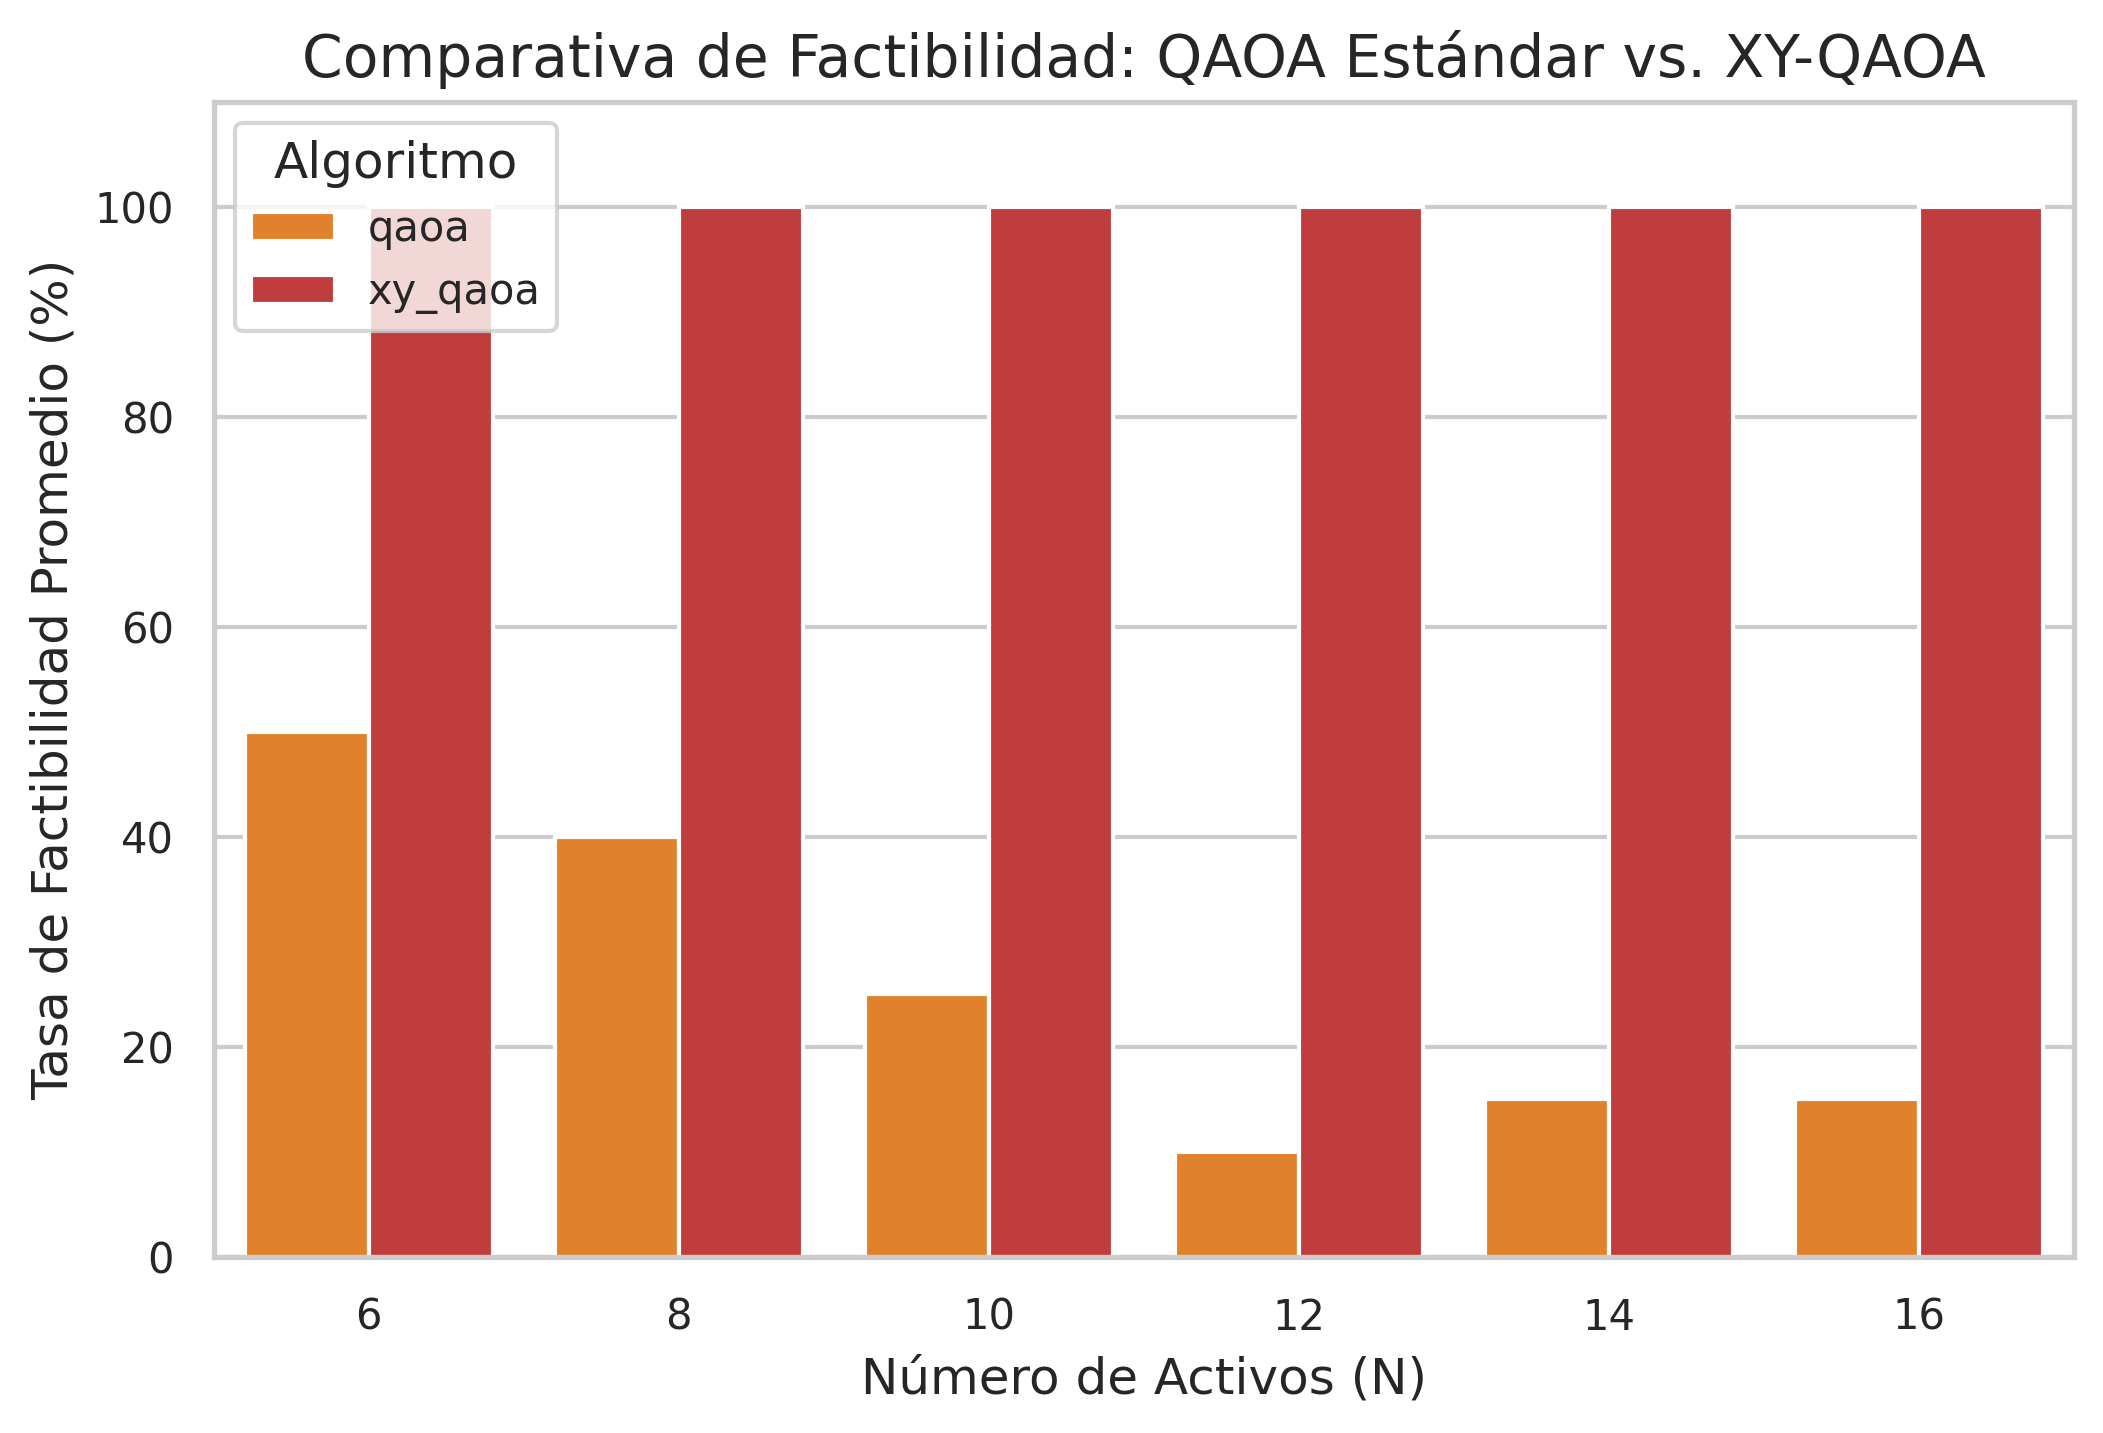
\includegraphics[width=0.85\textwidth]{output/figures/xy_vs_qaoa_feasibility.png}
    \caption{Comparación geométrica sobre el hipercubo booleano de $N=3$ cúbits con cardinalidad $K=1$. El QAOA estándar (izquierda) recorre la totalidad de los ocho vértices del hipercubo, seis de ellos infactibles. El XY-QAOA (derecha) confina la evolución al plano triangular formado exclusivamente por los tres vértices factibles.}
    \label{fig:hipercubo_feasibility}
\end{figure}

Finalmente, la topología completa del circuito propuesto, que intercala la inicialización determinista en el estado de Dicke con capas sucesivas de los operadores $U_C(\gamma)$ y $U_M^{XY}(\beta)$, se ilustra en la Figura \ref{fig:topologia_xy}.

\begin{figure}[htbp]
    \centering
    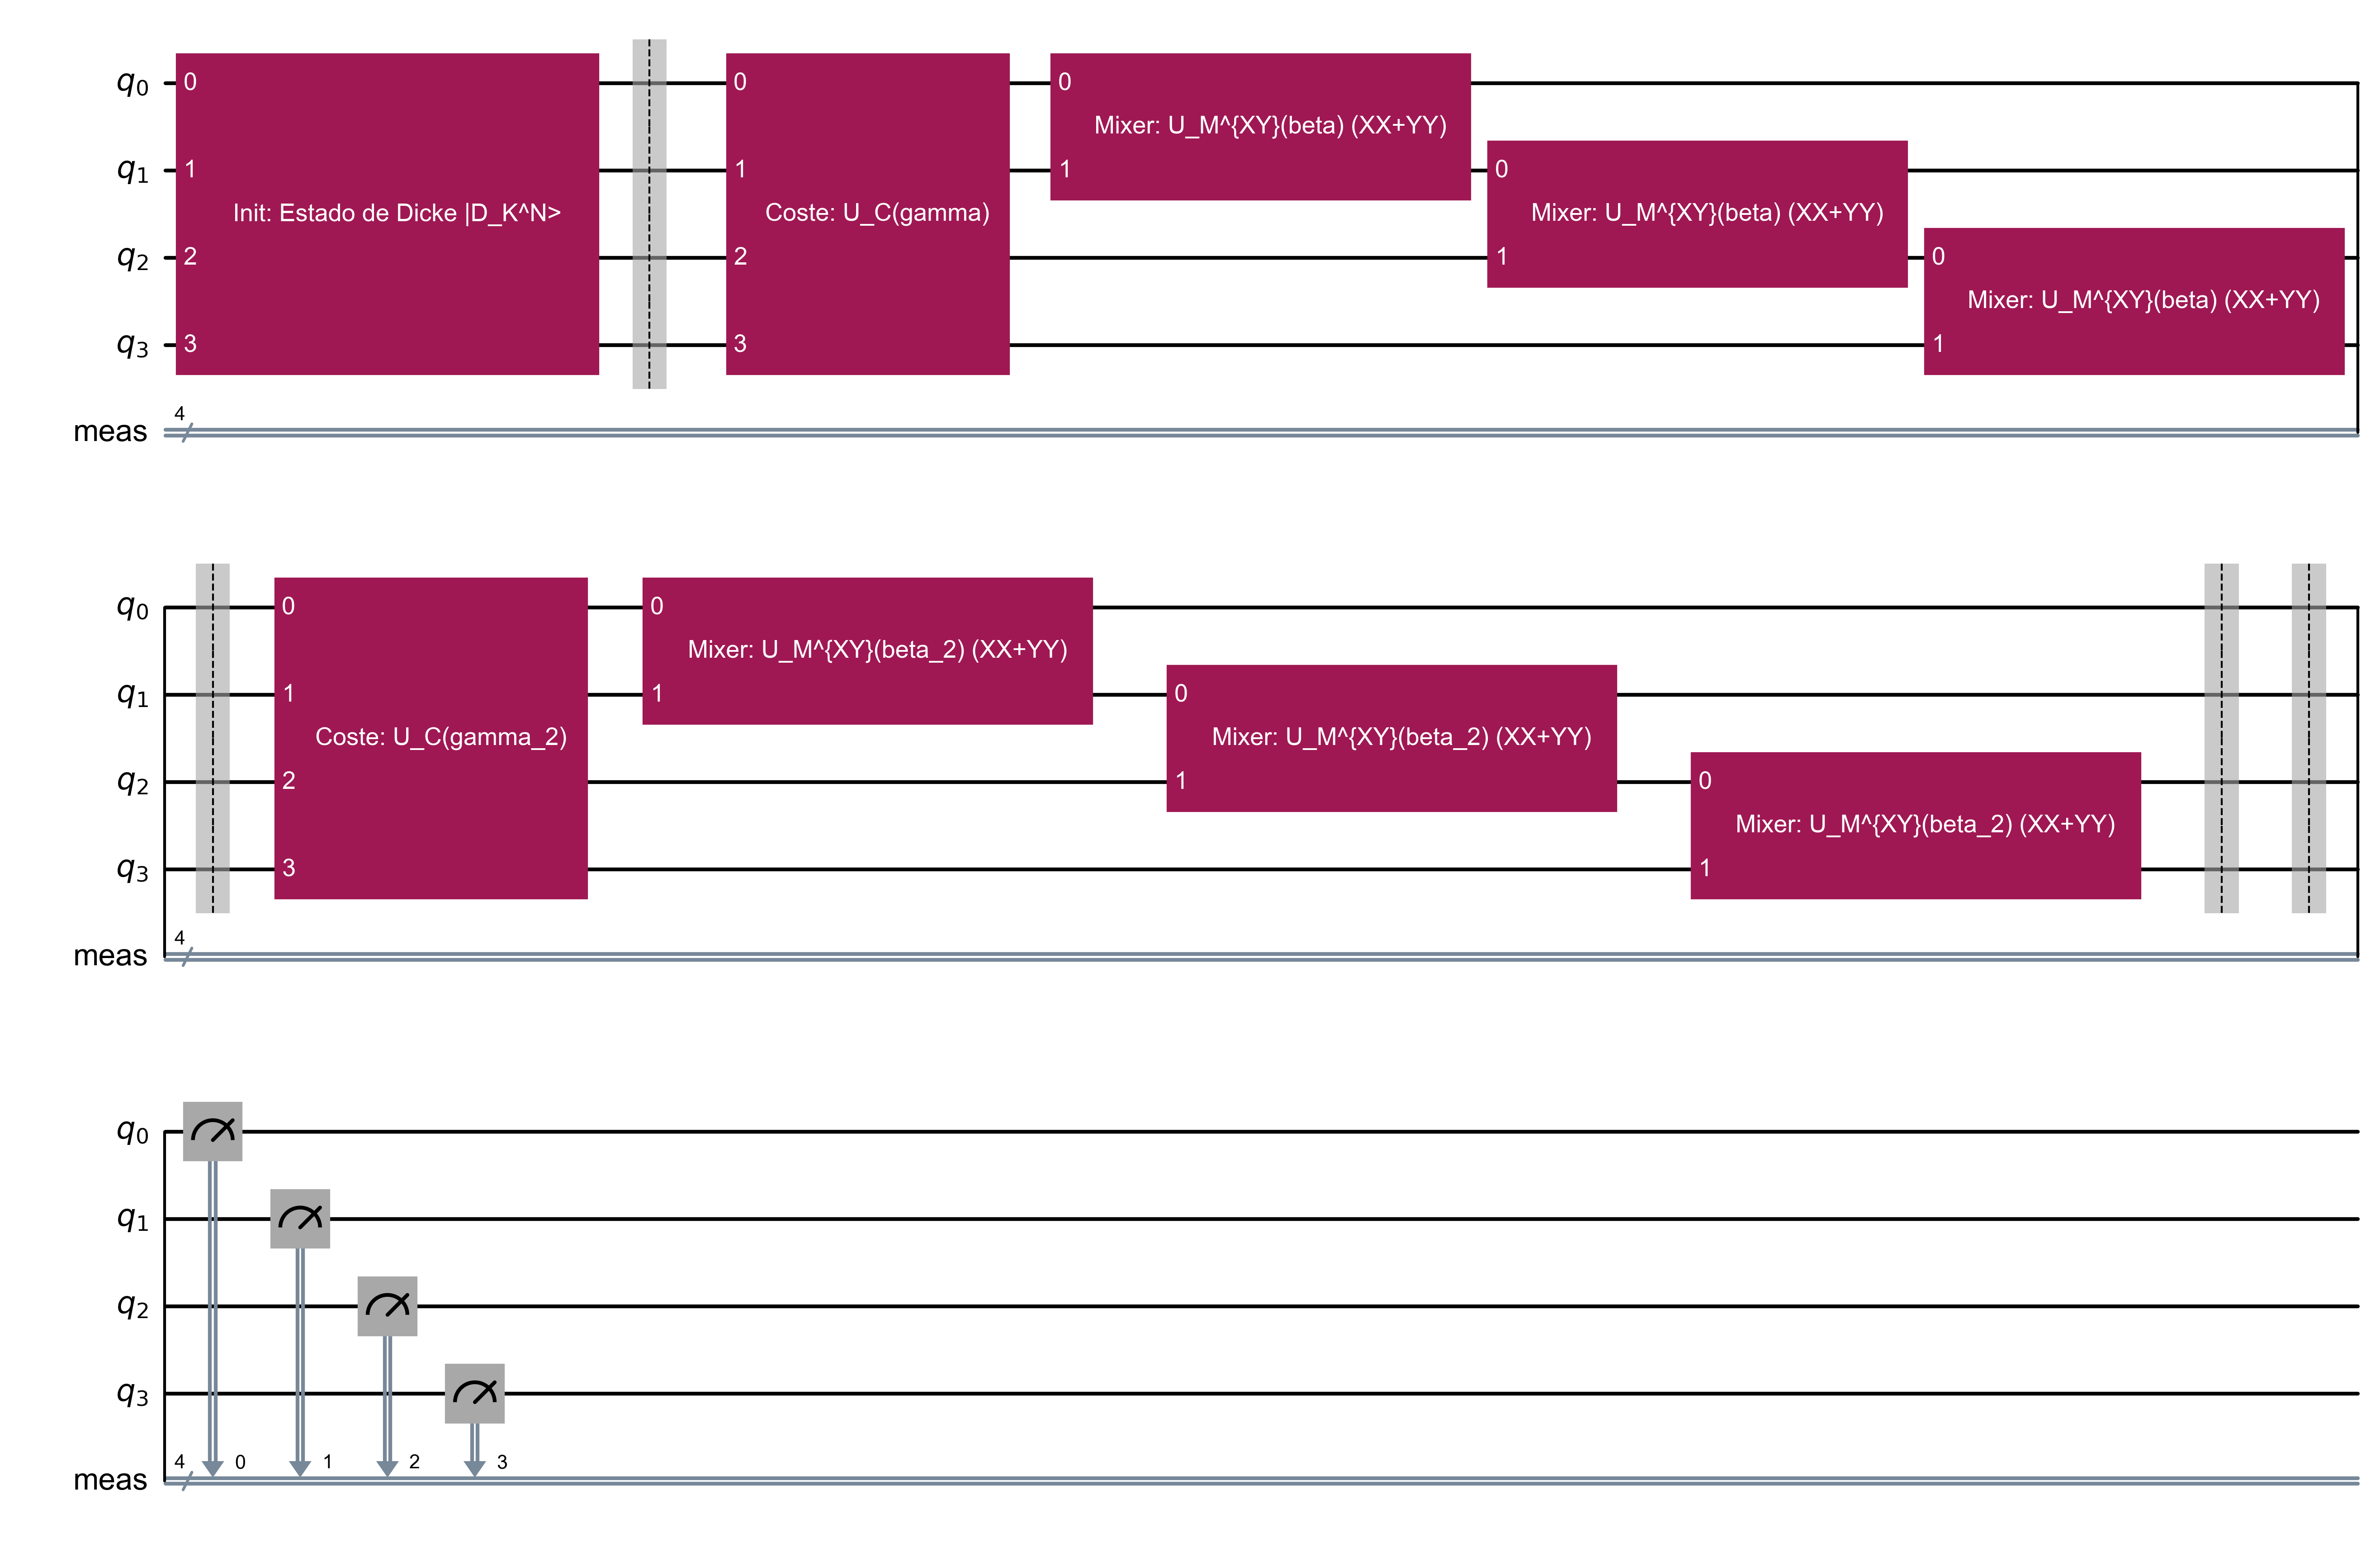
\includegraphics[width=0.85\textwidth]{output/figures/topologia_circuito_xy.png}
    \caption{Topología general del circuito cuántico XY-QAOA: inicialización determinista en el estado de Dicke, seguida por la aplicación iterativa de los operadores de coste $U_C(\gamma)$ y los operadores de mezcla con preservación de peso de Hamming $U_M^{XY}(\beta)$.}
    \label{fig:topologia_xy}
\end{figure}

\section{Estabilización del Paisaje de Optimización Clásica}
\label{sec:estabilizacion_optimizacion}

Aunque la arquitectura XY-QAOA descrita en la Sección \ref{sec:arquitectura_cuantica} resuelve por construcción el problema de la factibilidad de las soluciones, el paisaje energético $\langle H_P \rangle(\gamma, \beta)$ que debe recorrer el optimizador clásico puede seguir presentando una elevada rugosidad y una fuerte dependencia respecto a la inicialización de los parámetros variacionales, especialmente en instancias con un alto grado de correlación entre activos financieros. Para mitigar esta problemática, se incorporan dos mecanismos de estabilización complementarios.

\subsection{Trotterized Quantum Annealing (TQA)}
\label{subsec:tqa}

En lugar de inicializar los parámetros del circuito $(\gamma, \beta)$ de forma aleatoria, este trabajo emplea un esquema de inicialización basado en \textit{Trotterized Quantum Annealing} (TQA), que emula un proceso de recocido cuántico adiabático mediante una discretización lineal de la rampa temporal de evolución. Concretamente, para una profundidad de circuito $p$, los ángulos iniciales de cada capa $m = 1, \dots, p$ se calculan como:
\begin{equation}
    \gamma_m = \left(\frac{m}{p}\right) \Delta t, \qquad
    \beta_m = \left(1 - \frac{m}{p}\right) \Delta t
    \label{eq:tqa_schedule}
\end{equation}
donde $\Delta t$ actúa como un parámetro de escala temporal global del proceso de recocido simulado. En la práctica, el procedimiento habitual consiste en evaluar la energía esperada del circuito para un conjunto discreto de valores candidatos de $\Delta t$ y seleccionar aquel que produce la menor energía antes de dar comienzo al bucle de optimización clásica propiamente dicho. Es importante señalar que este esquema de inicialización TQA no sustituye a la optimización clásica posterior mediante COBYLA o SLSQP, sino que proporciona un punto de partida informado que, a diferencia de una inicialización aleatoria, se sitúa en una región del paisaje energético próxima a la trayectoria adiabática teórica del sistema.

\subsection{Regularización Ridge $L_2$}
\label{subsec:ridge_l2}

Como segundo mecanismo de estabilización, se integra una penalización continua de tipo Ridge ($L_2$) directamente en la función de coste clásica que evalúa el optimizador durante el bucle variacional. Denotando por $\theta = (\gamma, \beta)$ el vector completo de parámetros del circuito y por $\theta^{\text{TQA}}$ el ancla obtenida mediante el procedimiento descrito en la Sección \ref{subsec:tqa}, la función de coste regularizada se define como:
\begin{equation}
    \mathcal{L}_{\text{Ridge}}(\theta) = \langle H_P \rangle_\theta +
    \alpha \sum_{k} \left( \theta_k - \theta_k^{\text{TQA}} \right)^2
    \label{eq:ridge_regularizacion}
\end{equation}
donde $\alpha \geq 0$ es el coeficiente de regularización. Geométricamente, este término adicional introduce una componente de convexidad local centrada en el ancla TQA, actuando como un filtro de suavizado que penaliza las trayectorias de optimización que se alejan sustancialmente de dicha región de referencia, mitigando así el riesgo de que el optimizador clásico quede atrapado en mínimos locales espurios inducidos por el ruido estadístico del muestreo cuántico.

La elección del coeficiente $\alpha$ está sujeta a un compromiso de sesgo-varianza inherente al propio mecanismo de regularización: un valor de $\alpha$ excesivamente elevado ancla la solución final demasiado cerca del punto TQA inicial, introduciendo un sesgo que puede impedir que el optimizador explore soluciones de menor energía; por el contrario, un valor de $\alpha$ excesivamente bajo resulta insuficiente para estabilizar la convergencia frente a la varianza del paisaje. El valor concreto de $\alpha$ empleado en las instancias experimentales, así como la justificación empírica de dicha elección, se presentan en el Capítulo \ref{cap:desarrollo_metodologia}. El efecto geométrico cualitativo de esta regularización sobre el paisaje de coste se ilustra en la Figura \ref{fig:paisaje_ridge}.

\begin{figure}[htbp]
    \centering
    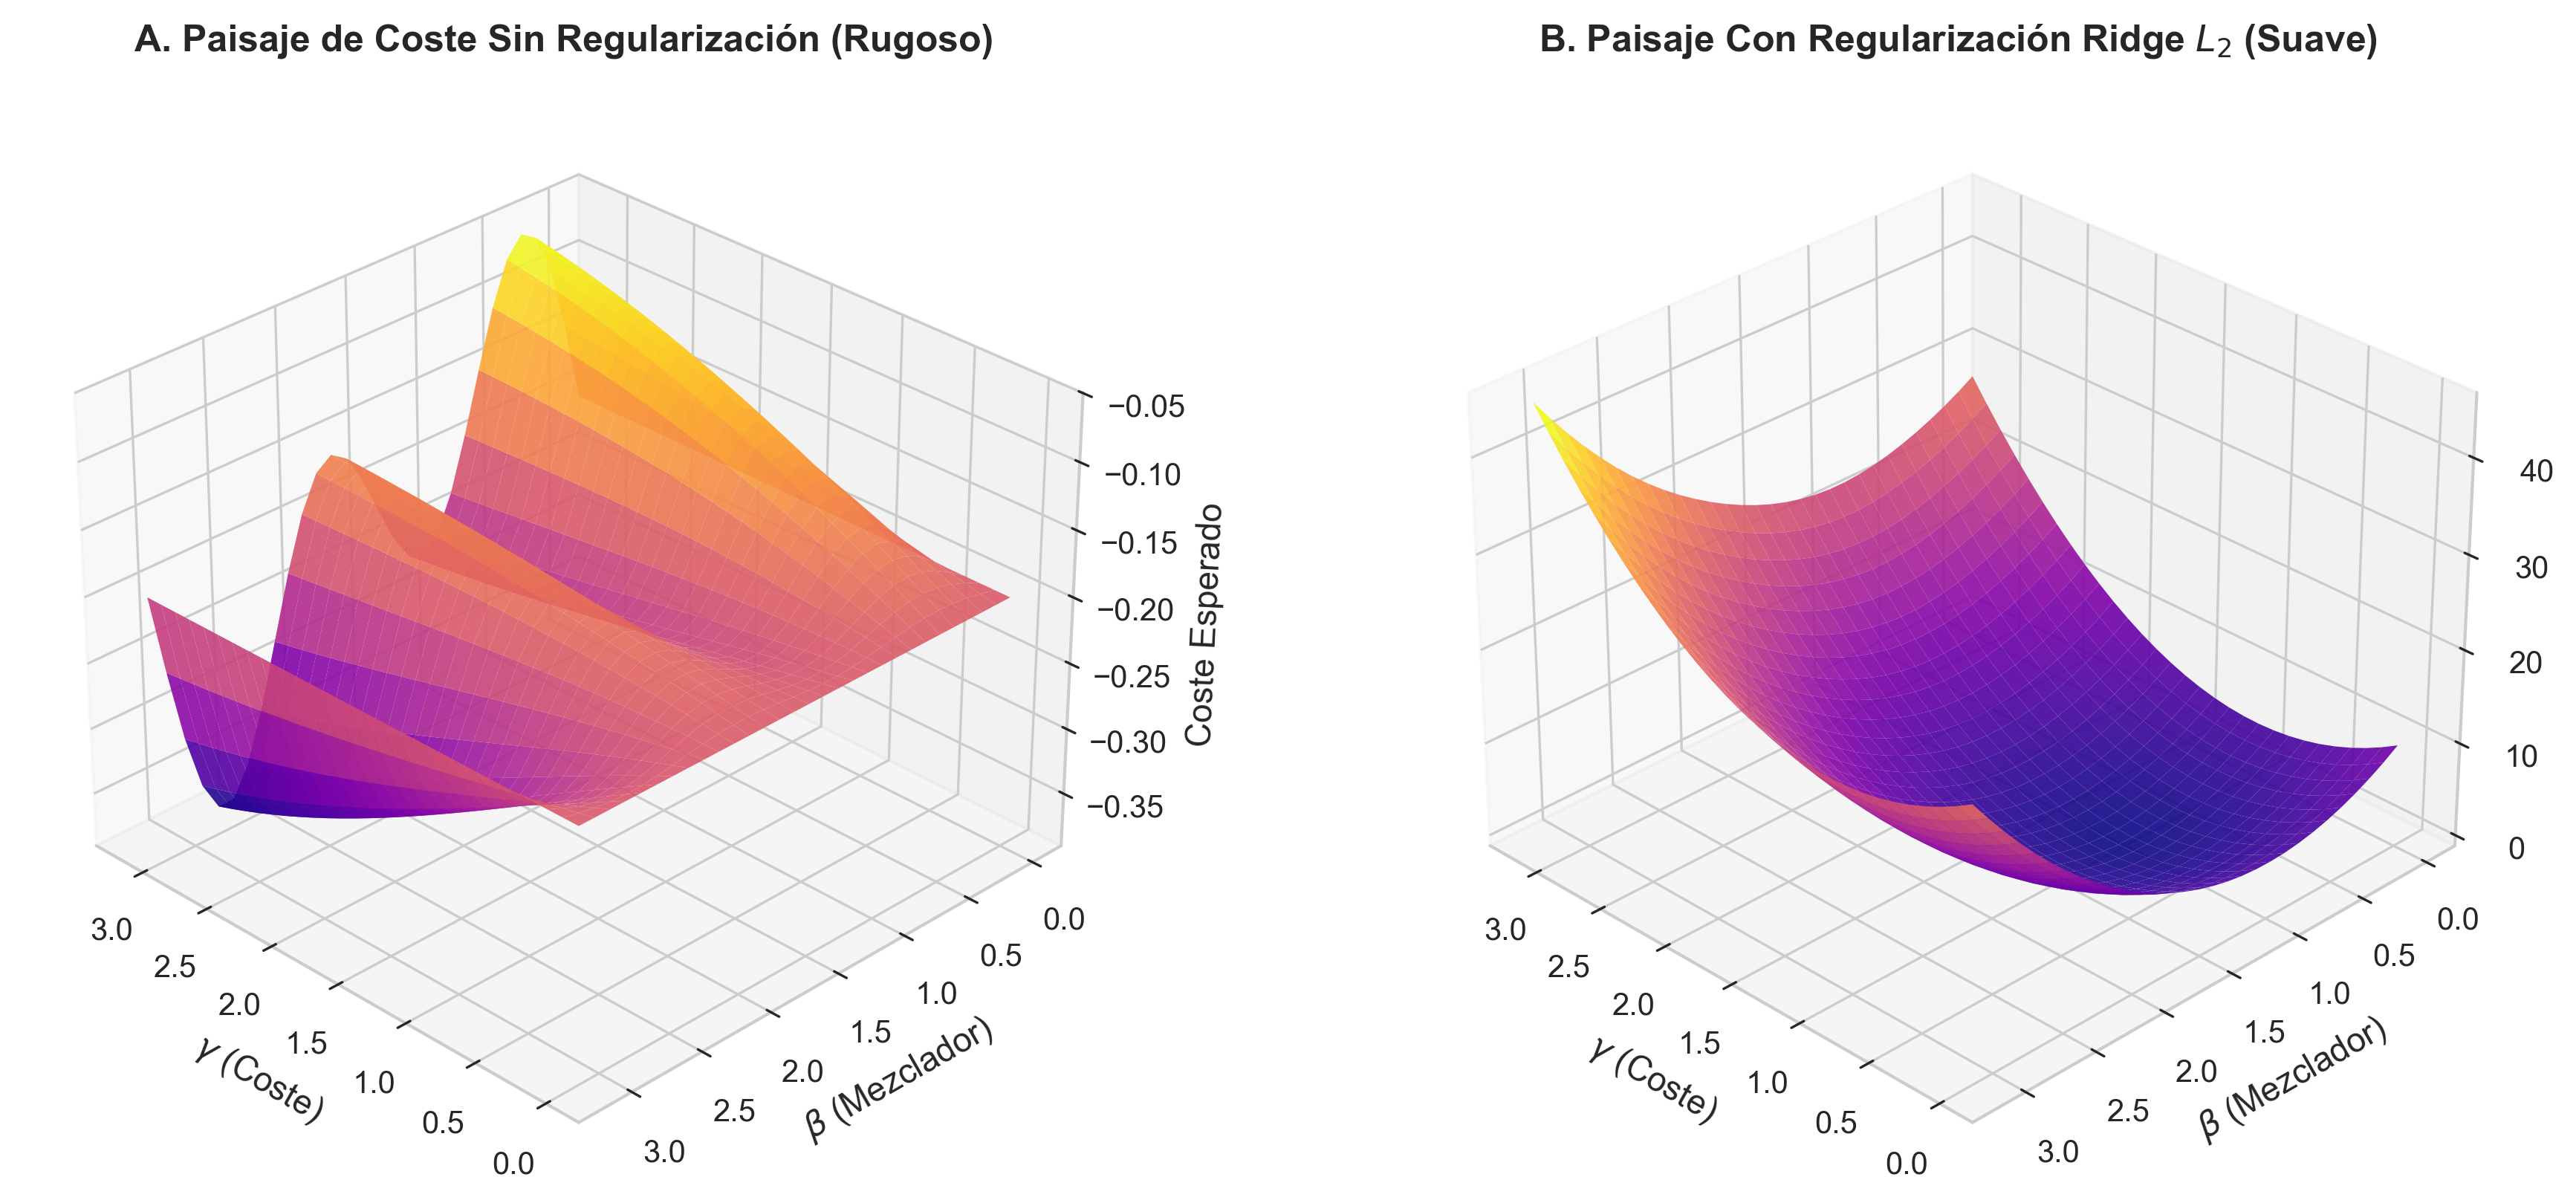
\includegraphics[width=0.9\textwidth]{output/figures/paisaje_regularizacion_ridge.png}
    \caption{Efecto analítico de la regularización Ridge $L_2$ en el paisaje de energía de la función de coste. (Conceptual)}
    \label{fig:paisaje_ridge}
\end{figure}